\documentclass[journal]{IEEEtran}
\usepackage[spanish,english]{babel}

\usepackage{amssymb, amsmath} %Paquetes matemáticos de la American Mathematical 
\usepackage[utf8]{inputenc}
\usepackage{graphicx}
\usepackage{float}
\usepackage{hyperref}
\usepackage{listings}
\usepackage{xcolor}

\definecolor{codegreen}{rgb}{0,0.6,0}
\definecolor{codegray}{rgb}{0.5,0.5,0.5}
\definecolor{codepurple}{rgb}{0.58,0,0.82}
\definecolor{backcolour}{rgb}{0.95,0.95,0.92}
% Definicio de estilo para el codigo fuente que se cita
\lstdefinestyle{mystyle}{
    backgroundcolor=\color{backcolour},   
    commentstyle=\color{codegreen},
    keywordstyle=\color{magenta},
    numberstyle=\tiny\color{codegray},
    stringstyle=\color{codepurple},
    basicstyle=\ttfamily\footnotesize,
    breakatwhitespace=false,         
    breaklines=true,                 
    captionpos=b,                    
    keepspaces=true,
    numbers=left,                    
    numbersep=5pt,                  
    showspaces=false,                
    showstringspaces=false,
    showtabs=false,                  
    tabsize=2,
}
\lstset{style=mystyle}

\renewcommand{\lstlistingname}{Código}

\begin{document}

\title{Ejercicio 4 - tema 2 \\ Administración de parámetros}
%
\author{Vicente Romero Andrade}

\markboth{Ejercicio 4 - tema 2 Administración de parámetros, Abril~2021}%
{Shell \MakeLowercase{\textit{et al.}}: }
% The only time the second header will appear is for the odd numbered pages

\maketitle


\IEEEpeerreviewmaketitle

\section{Objetivo}
% The very first letter is a 2 line initial drop letter followed

\IEEEPARstart{E}{l} objetivo es comprender y poner en práctica los conceptos asociados con la configuración de los 
parámetros de una base de datos, en particular, los 3 niveles de aplicación: nivel sesión, nivel instancia y nivel SPFILE, 
así como las diferentes opciones que existen para obtener y reconstruir tanto PFILEs como SPFILEs.


\section{Desarrollo}
\subsection{C1. Contenido del script s-00-crea-directorios.sh}
\lstinputlisting[language=bash,caption=s-00-crea-directorios.sh,label={lst:scriptloop}]{s-00-crea-directorios-root.sh}
\subsection{C2. Contenido del archivo e-01-spparameter-alert-log.txt}
\lstinputlisting[caption=e-01-spparameter-alert-log.txt,label={lst:scriptpwd}]{e-01-spparameter-alert-log.txt}
\subsection{C3. Contenido del script s-01-spparameters.sql}
\UseRawInputEncoding
\lstinputlisting[language=sql,caption= s-01-spparameters.sql,label={lst:scriptpwd}]{s-01-spparameters.sql}
\subsection{C4. Contenido parcial del archivo e-03-spparameter-pfile.txt}
\lstinputlisting[language=sql,caption=e-03-spparameter-pfile.txt,label={lst:scriptpwd}]{e-03-spparameter-pfile.txt}
\subsection{C5. Salida del validador de cambio de parámetros}
\begin{figure}[H]
  \centering
  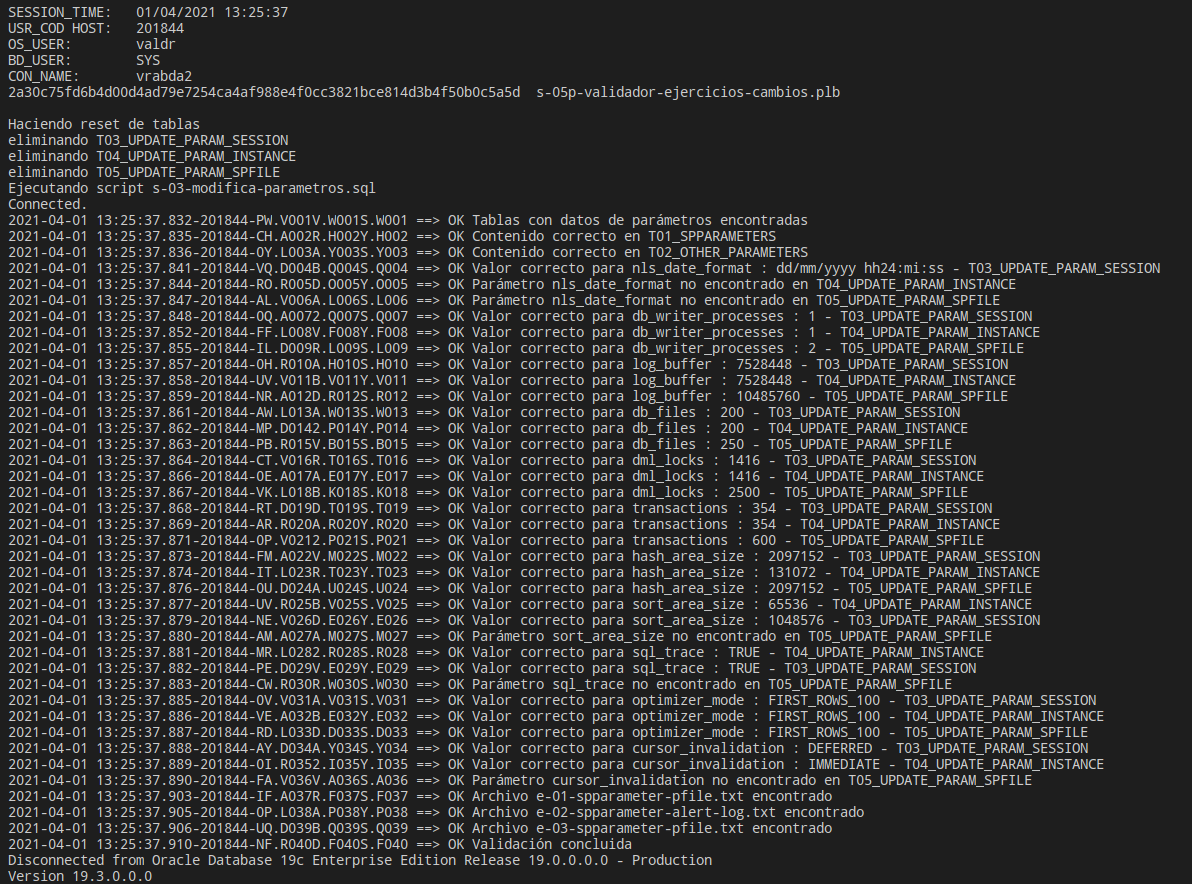
\includegraphics[scale=.21]{t020401.png}
   \caption{Salida del validador cambio de parametros}
   \label{fig:salidascript}
\end{figure}
\subsection{C6. Salida del validador de restauración de parámetros}
\begin{figure}[H]
  \centering
  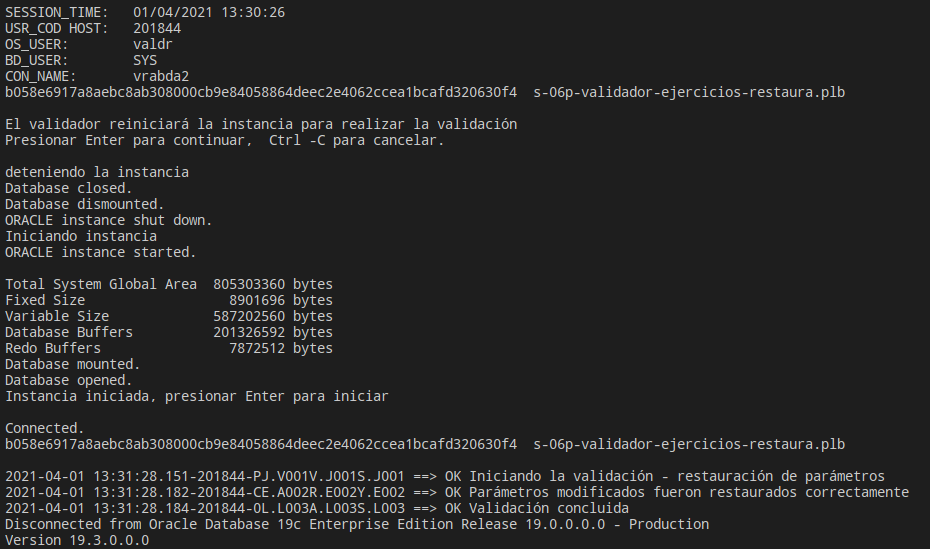
\includegraphics[scale=.25]{t020402.png}
   \caption{Salida del validador restauración de parametros}
   \label{fig:salidascript}
\end{figure}

\section{Conclusiones}
En este ejercicio práctico se vio el proceso para poder configurar los parámetros 
de configuración de la base de datos, tanto la forma para hacerlo de forma persistente
como para solo hacerlo durante la instancia o sesión. Adicionalmente se vio la forma de 
poder generar respaldos de estas configuraciones y el como se pueden restaurar en caso de que 
algo salga mal.
\ifCLASSOPTIONcaptionsoff
  \newpage

\fi
\end{document}
